\subsection{Overview}
Given the nature of the application, a three layer approach has been chosen.\newline
\begin{figure}[h!]
	\centering
	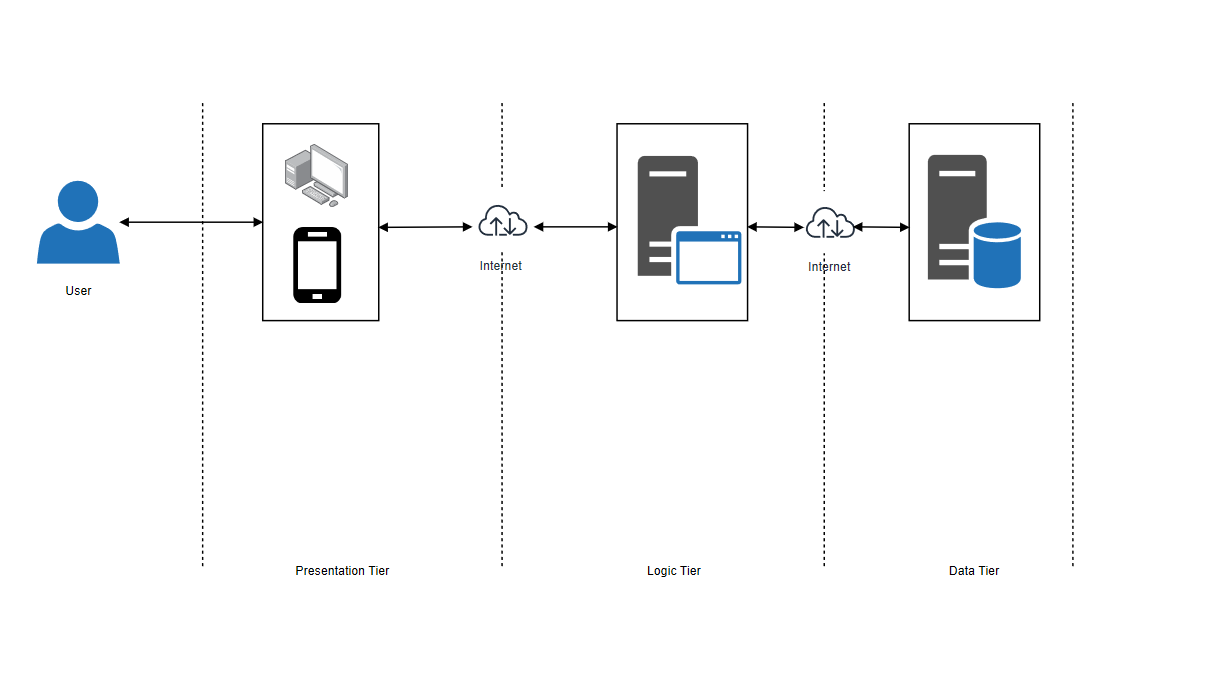
\includegraphics[width=\textwidth]{Images/three_layer}
	\caption{Three layer structure}
\end{figure}
\newline
As shown by the image above, the three layers consist in the presentation tier, the logic tier and the data tier
\begin{itemize}
\item Presentation Tier: consists of the user interfaces for all of the three clients (RegularUser, Policeman and MunicipalAuthority) and is used by the user to interact with both the application logic and Google Mapd APIs \newline
\item Logic Tier: consists of the servers used to control the functionalities of the application, interacts with both the presentation and data tiers \newline
\item Data Tier: consists of the database server (where both user data and data generated by the application are stored), interacts only with the logic tier \newline
\end{itemize}
\newpage
\subsection{Component view}
\subsubsection{Introduction}
The following diagram represents the interface structure of the system, focusing on the application server structure. \newline
\begin{figure}[h!]
	\centering
	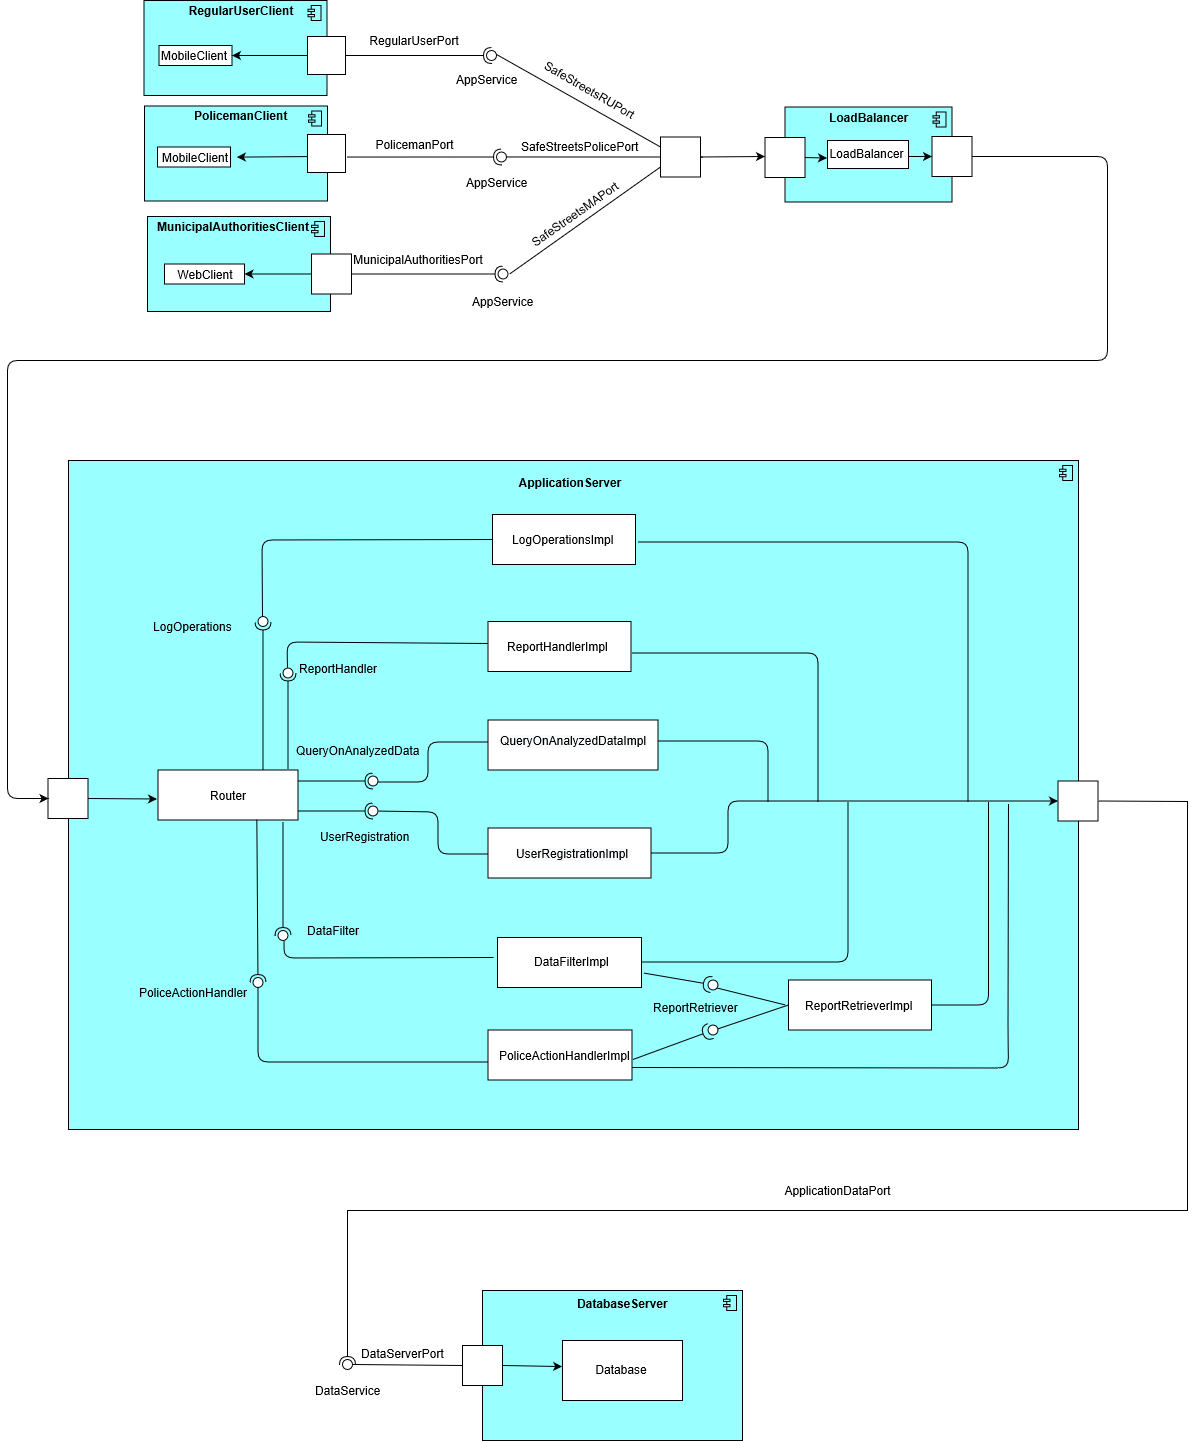
\includegraphics[width=\textwidth]{Images/component_diagram_beta}
	\caption{Component diagram}
\end{figure}

As shown above, the application logic is stored on the application server, while the clients just contain what is mandatory in order to contact the application server (thin client).\\
\subsubsection{Server}
We will now proceed to give a brief summary of the role of the components listed above:
\begin{itemize}
\item QueryOnAnalizedData: allows the RegularUser profiles to access data about the reports in a certain area or other information already analized by the MunicipalAuthorities
\item PoliceAction: allows the policemen to take action on user made reports or to compile reports themself. The actions performed by the police consist in compiling reports (of which they will take care right away), marking themselves as dispatched towards a report, mark a report as wrong or signal that a traffic ticket has been written as a consequence of a reported traffic violation
\item RetrieveEquiReports: this component is used by PoliceAction and QueryOnData in order to retrive all reports that are about the same violation (not just violation type, but also time, plate and location) as a given one. 
\item SendReports: this component allows users to submit the reports about traffic violations that they write. The reports are authenticated and then strored inside the application DB
\item UserRegistration: this component allows the registration of all types iof users. Note that, while RegularUser profiles registration is done by the user themselves, Authority profiles (Policeman and MunicipalAuthority) can only be registered by a system admin
\item LogOperations: this component takes care of the login and logut operations for all types of User profiles
\item QueryOnData: allows MunicipalAuthority profiles to perform data-mining activities,  as well as add information from the municipality DB of crashes and cross-analyze them with user-submitted reports
\end{itemize}
The logic of the application works based on the afromentioned components: they grant all the functionality needed to satisfy the system's goals (for a more in-depth analysis see chapter 4).
In the next two pictures more information about the system will be provided via a more accurate version of the class diagram presented in the RASD and a schema about the relationship between the classes interfaces and implementations of said interfaces. Please note that the "Device" class and the classes that extend it are not reported in the diagram since they are not relevant to the purposes of this description. For any further information about these classes refer to the Class diagram in the RASD.

\begin{figure}[h!]
	\centering
	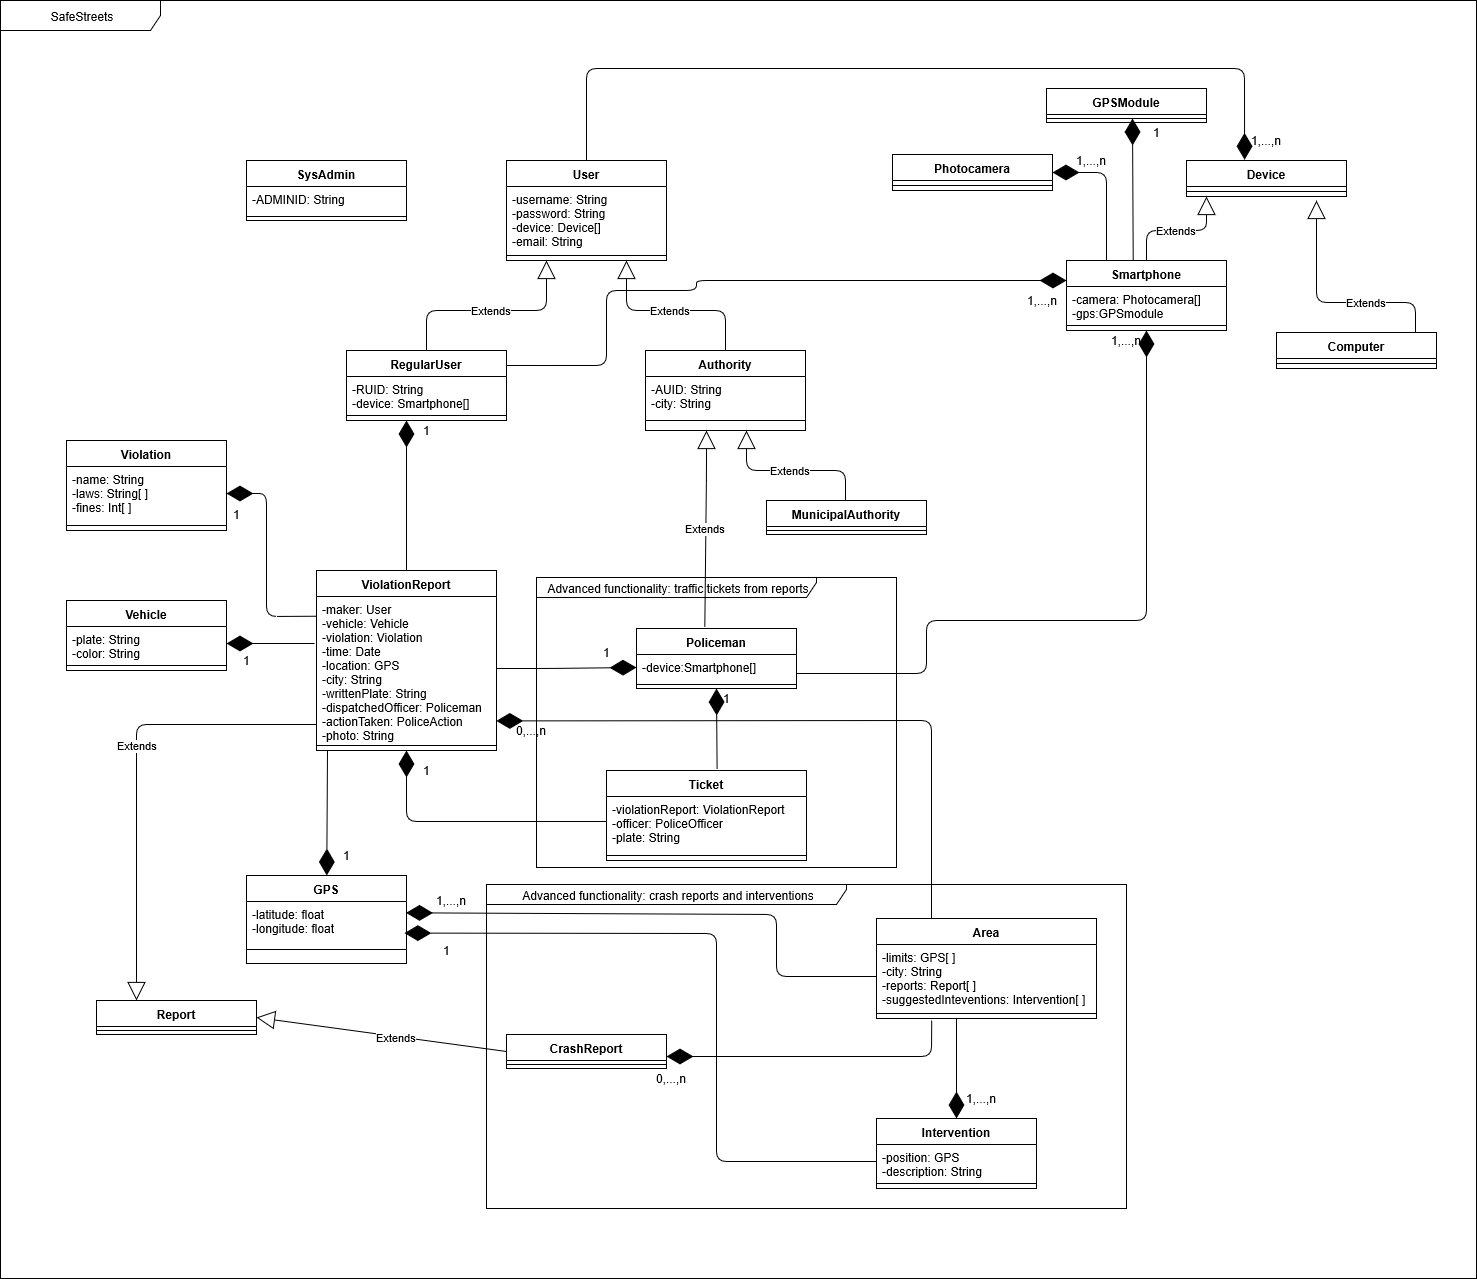
\includegraphics[angle=90, scale=0.40]{Images/ADV_class_diagram}
	\caption{Class diagram}
\end{figure}
\newpage

\begin{figure}[h!]
	\centering
	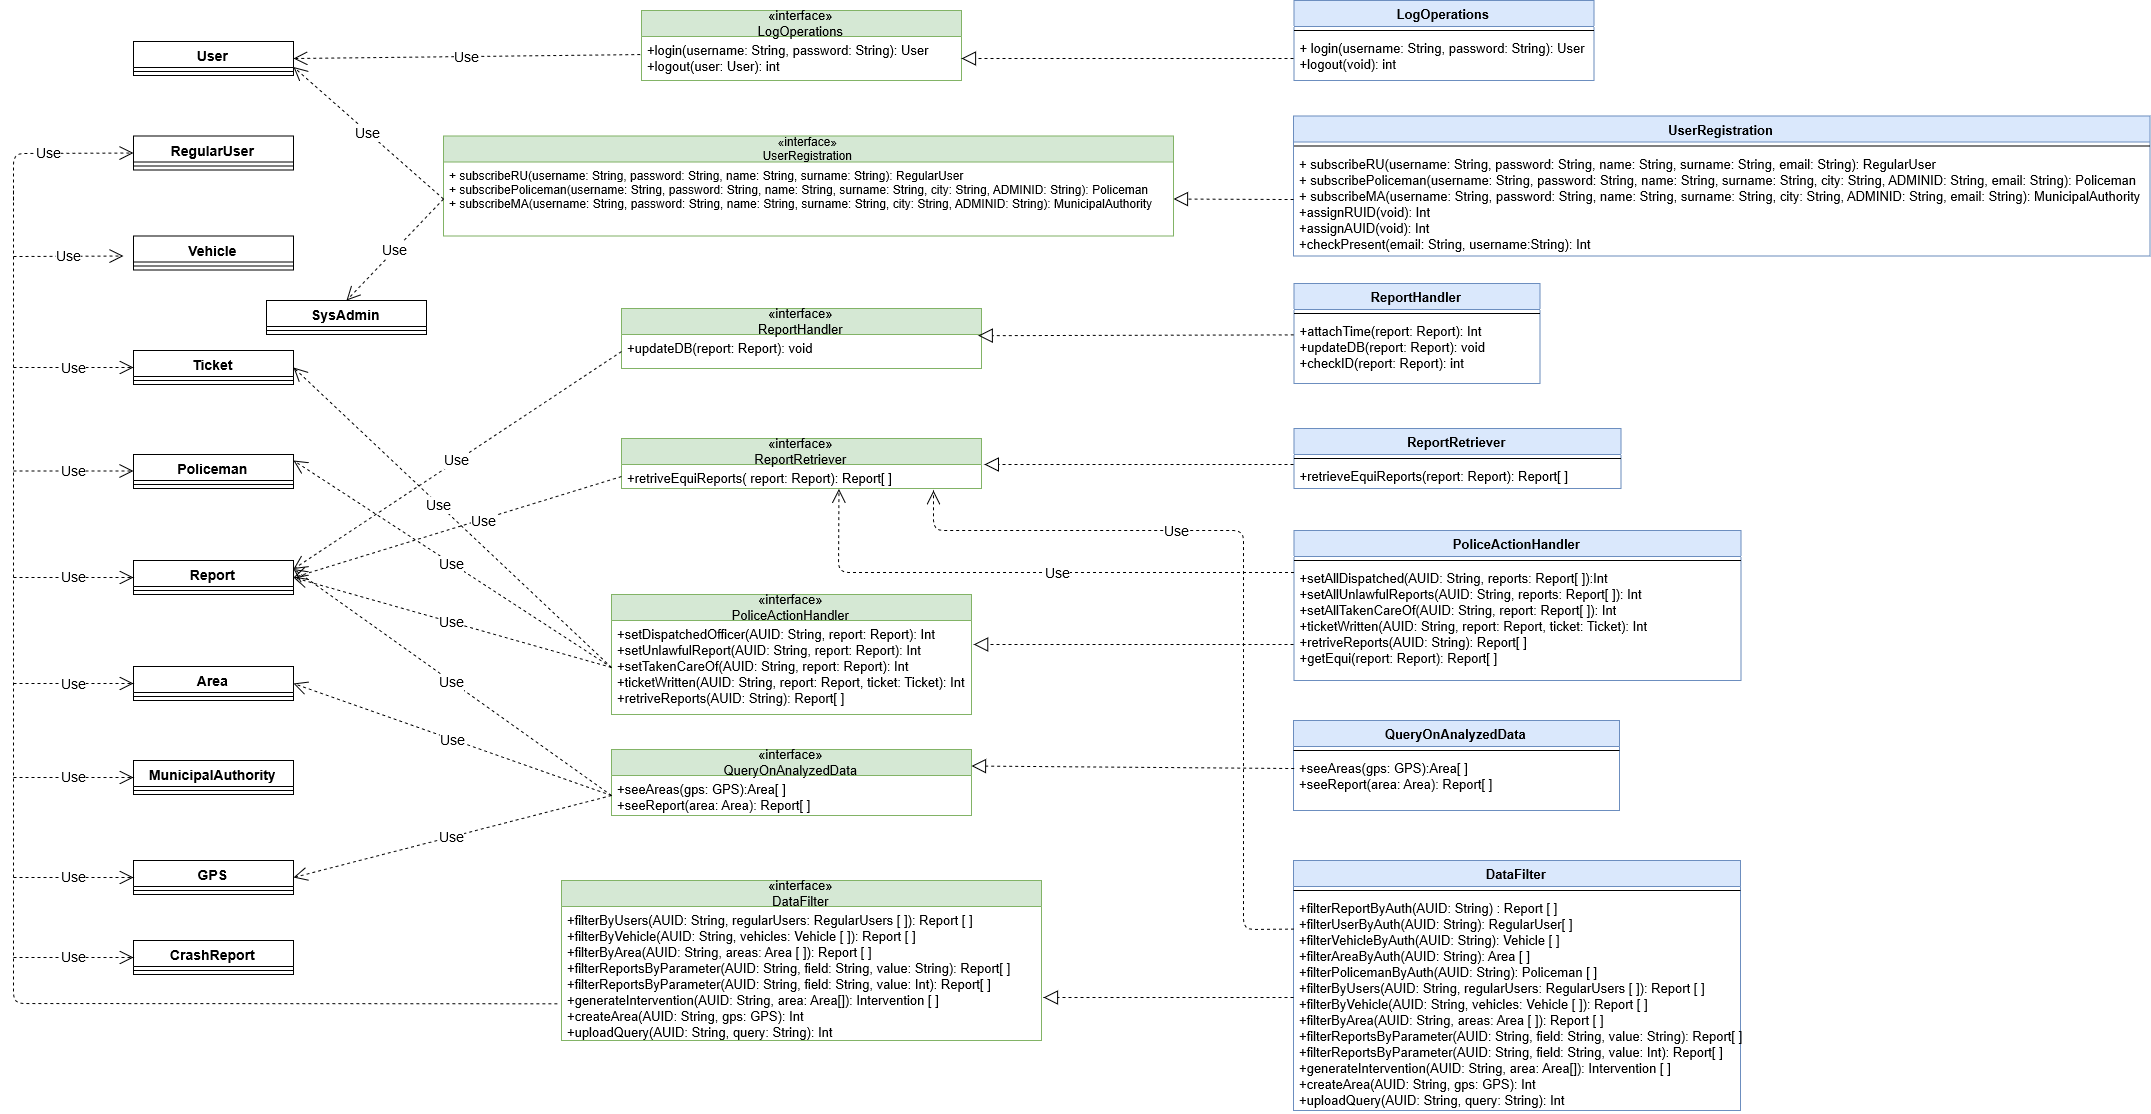
\includegraphics[angle=90, scale=0.25]{Images/component_class_relation}
	\caption{Relation between components and already specified classes}
\end{figure}
\newpage
\subsubsection{Client}
In this section, we will give a description of the three clients functions showed in the introduction:
\begin{itemize}
	\item RegularUserClient: allows regular users to register and login to the service, to send reports about traffic violations and visualize on a map the most unsafe areas around him.
	\item PolicemenClient: allows policemen login to the service, to retrieve reports sent by the regular users and to communicate that they are working to resolve a specific report.
	\item MunicipalAuthoritiesClient: allows municipal authorities login to the service, to mine data about their municipality from the DataBase and to cross data about accidents with the informations collected by SafeStreets.
\end{itemize}
In the following pictures we will provided more detailed informations about the three clients' components, focusing on one at a time.

\begin{figure}[h!]
	\centering
	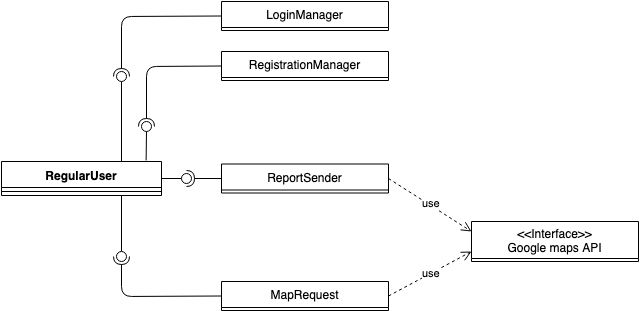
\includegraphics[scale=0.7]{Images/RegularUserClient}
	\caption{Relation between components inside regular user client}
\end{figure}
The components represented in this diagram are:
\begin{itemize}
	\item SendLogData: Allows users to send their log data to the server in order to login or logout from the system.
	\item SendRegistrationData: Allows users to send  their registration data to the server in order to register a new account.
	\item SendReport: Allows users to send a report about traffic violations and all the required data to the server.
	this component also uses Google maps API in order to recover informations about the area around user's geographical position.
	\item MapRequest: Allows the user to visualize a geographical map from Google maps API enriched by data about unsafe areas, statistics and traffic violations coming from the server.
\end{itemize}

\begin{figure}[h!]
	\centering
	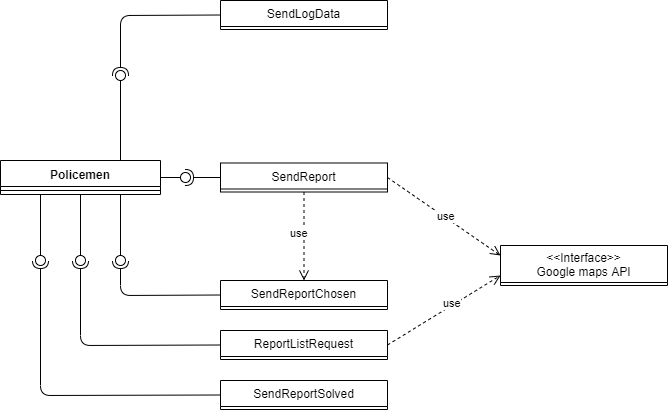
\includegraphics[scale=0.7]{Images/PolicemenClient}
	\caption{Relation between components inside policemen client}
\end{figure}
The components represented in this diagram are:
\begin{itemize}
	\item SendLogData: It has the same function as in the regular user client.
	\item SendReport: Allows Policeman to send a report about traffic violations and all the required data to the server.
	this component also uses Google maps API in order to recover informations about the area around user's geographical position.
	As seen in the diagram, the connection between SendReport and SendReportChosen means that, if a policeman sends a report about a violation, he is automatically assigned to solving it.
	\item ReportListRequest: Allows a policeman to request the list of the various pending reports around the municipality  he is in assigned.
	The location of the various reports will be shown on a map provided through Google maps API.
	\item SendReportChosen: Allows a policemen to send informations about the report he is going to solve.
	\item SendReportSolved: Allows a policeman to send informations about the report he just solved.
\end{itemize}

\begin{figure}[H]
	\centering
	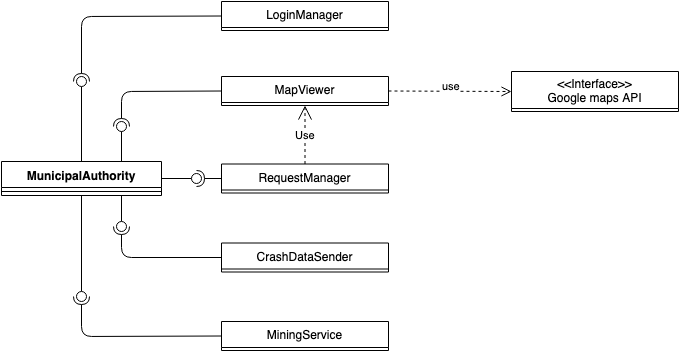
\includegraphics[scale=0.7]{Images/MunicipalAuthoritiesClient}
	\caption{Relation between components inside municipal authorities client}
\end{figure}
The components represented in this diagram are:
\begin{itemize}
	\item SendLogData: It has the same function as in the regular user client.
	\item DataRequest: Allows the municipality to request data about Reports(solved or not) from the server.
	The location of the various reports will be shown on a map provided through Google maps API.
	\item SendCrashData: Allows the municipal authority to send Data about car crashes around the municipality to the server in order to be crossed with data already collected.
	\item MineData: Allows the municipality to mine data collected by the server.
\end{itemize}

\newpage
\subsection{Deployment view}

\begin{figure}[h!]
	\centering
	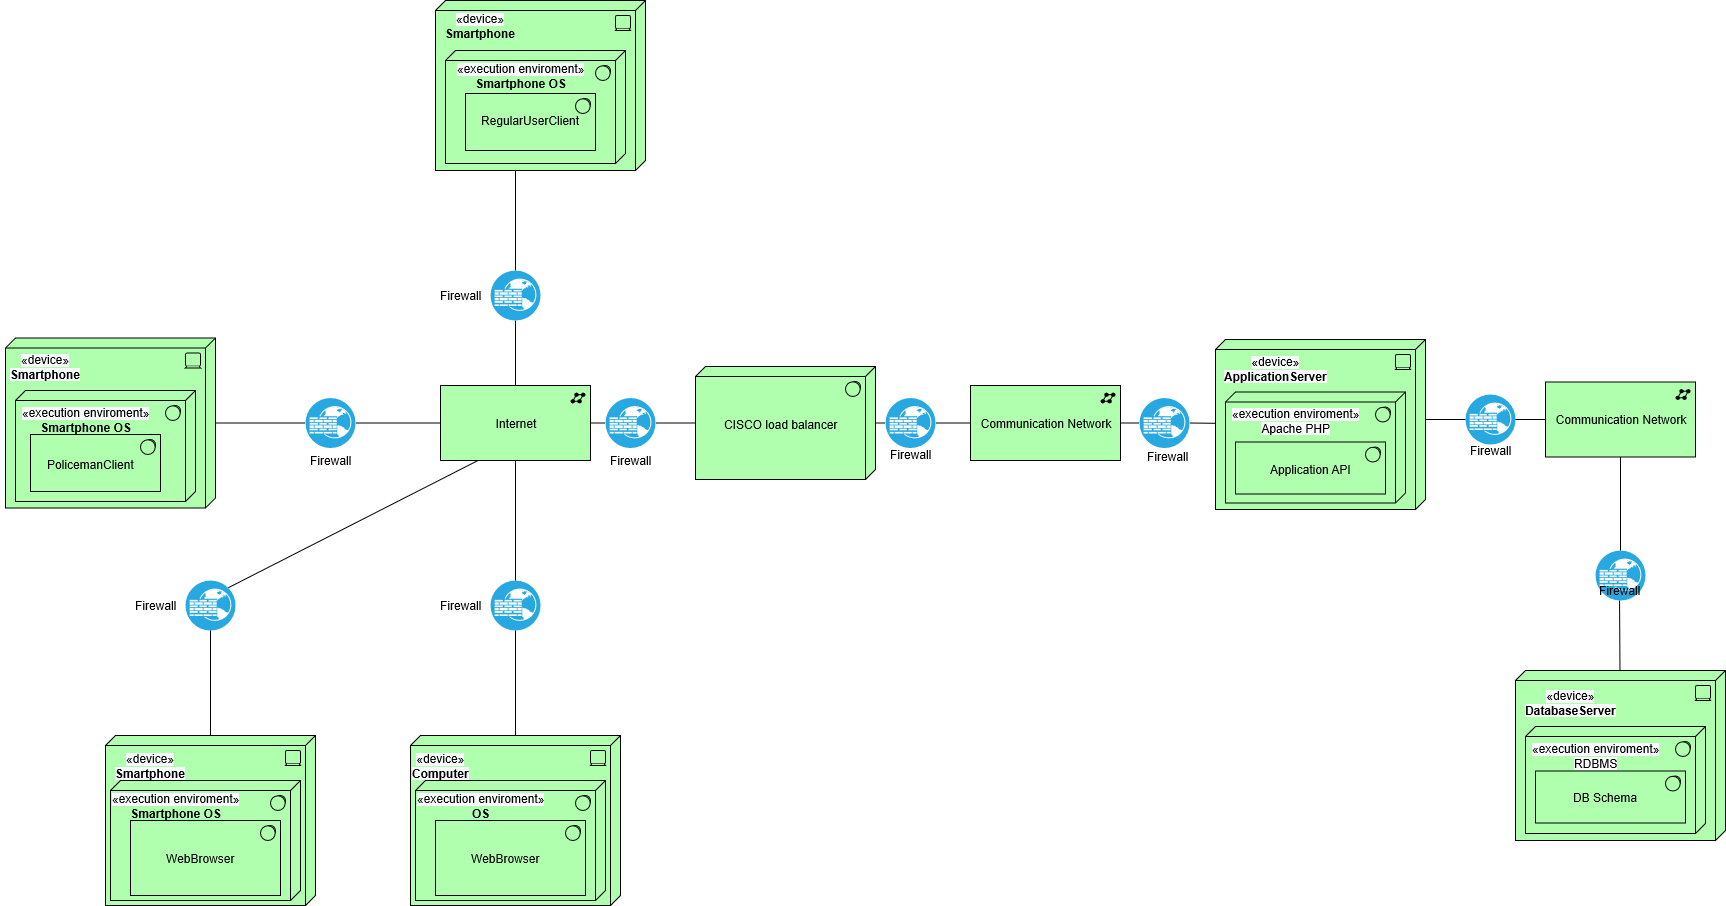
\includegraphics[width=\textwidth]{Images/physical_view}
	\caption{Physical view}
\end{figure}

The image above shows the system's architecture from a physical standpoint.
Components:
\begin{itemize}
\item Smartphone: Device used by both RegularUser and Policeman users type to interact with the application. Two different clients will be developed: one for regular users, that will allow them to look at already analyzed data and submit reports, and a different one for policemen, that will allow the officers make reports (upon which they will take actions right away) and take actions on reports
\item Computer: device used by MunicipalAuthorities users. They will interact with the application via a web page, that will allow them to interact in various ways with the Reports submitted by the other users.
\item Application server: this server contains the application logic and will interact with the different clients in a client-server way.
\item DatabaseServer: this server contains the actual data, both about the registered users and related to the user submitted reports, the actions taken by the police and the results of the data mining operations done by municipal authorities
\end{itemize}
Please note that Google servers have not been included, since those servers will not be involved in the system deployment
\newpage
\subsection{Runtime view}
\newpage
\subsection{Interfaces}
\begin{figure}[h!]
	\centering
	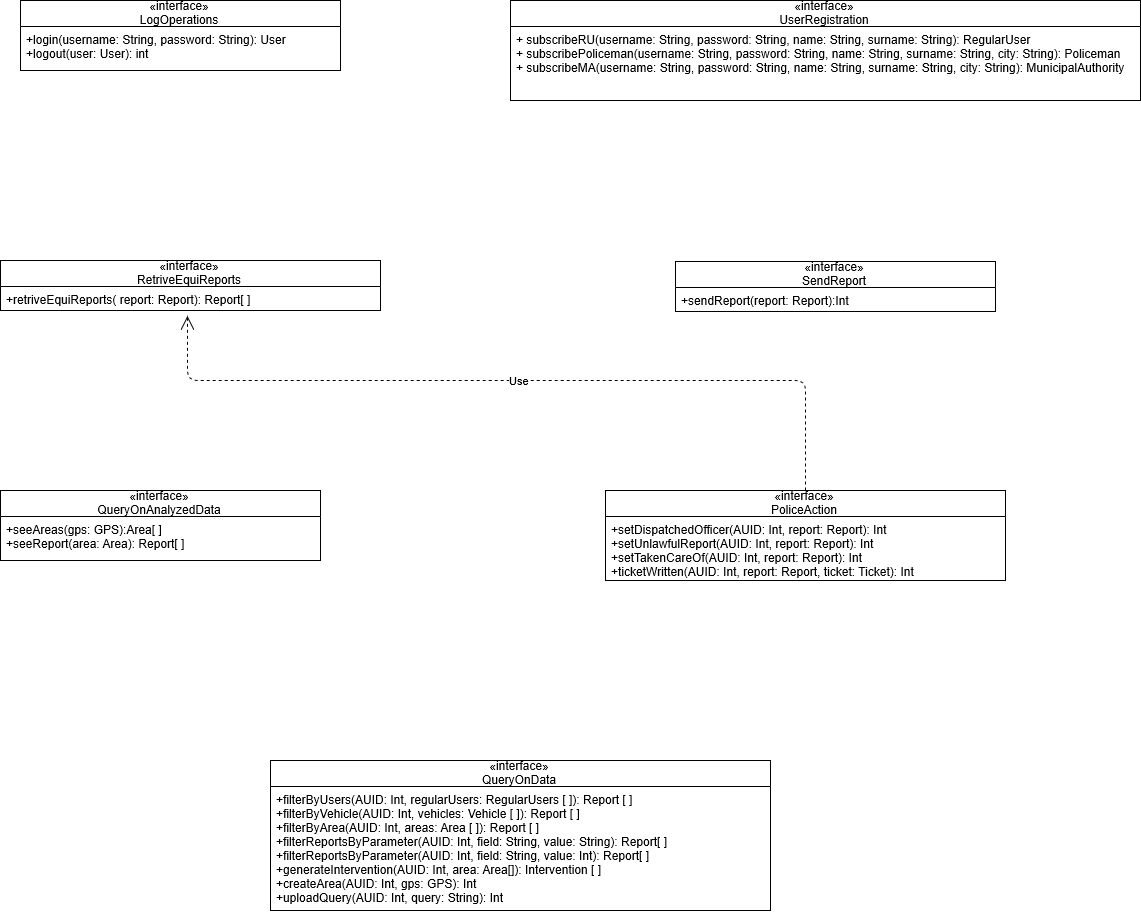
\includegraphics[width=\textwidth]{Images/interface_diagram}
	\caption{Components' interfaces}
\end{figure}
Other than the relation between PoliceAction, QueryOnData and RetriveEquiReports, already explained in section 2.2, it is worth noting that the interfaces don't actually expose all the methods of the objects that implement them. This choiche was made in order to hide the methods that will be colled only from inside the object in which they are defined.
\newpage 
\subsection{Architectural and implementative styles and patterns}
\subsubsection{Architectural styles}
\begin{itemize}
	\item Client-server:given the nature of the application, a distibuted system in which data submitted by some users has to be accessible by other users, the figure of a mediator becomes necessary. Therefore a client-server architecture seems is a good solution. Another alternative could have been cloud computing architecture (SaaS, flex tenacity approach), but we have chosen a client-server architecturesince the workload and scalability issues would not be big enough to justify the increased costs.
	\item Thin client: in the afromentioned client-server architecturethe role of the server is more than just a message manager. As a matter of fact, the server also takes care of the application logic, allowing a light client
	\item Three tiers architecture: given the client server with thin client architecture described, the most natural solution is a three tier architecture in which the presentation layer is on the client, the application layer on the application server and the data layer on the database server 
\end{itemize}
\subsubsection{Design patterns}
\begin{itemize}
	\item Model-view-controller: given the three-tiered and thin client architecture, using a MVC design pattern is quite easy: the model will be in the database server, the control in the application sserver and the view in the various clients
	\item Facade: used to hide the application server's components complexity
	\item Factory: used in RegularUser and Policeman clients to create reports
\end{itemize}
\subsection{Other design choiches}
\begin{itemize}
	\item Security concerns: as expressed in the RASD, there are various measures neede in order to obtain a good level of security:
	\begin{itemize}
		\item Fileting and escaping registartion requests of all kinds of user profiles and RegularUser submitted reports (Policeman submitted ones and MunicipalAuthority queries are considered trustwothy) in order to avoid code injections
		\item escaping and filetring login fields in order to avoid code injections
		\item all communication must happen over a secure channel (HTTPS)
		\item an anti cross site request forgery token is needed 
	\end{itemize}
	\item Database: for this application a relational database managemant system has been chosen
\end{itemize}